%! TeX program = lualatex
\documentclass[main]{subfiles}

\begin{document}

\title[AutoML: HPO]{Local Search and Ablation Analysis}
\subtitle{Adaptive Search and Hyperparameter Importance}
\author[Lars Kotthoff]{Lars Kotthoff}
\date{}

%\institute{}
%\date{}
	
	\maketitle
	

\begin{frame}{Local Search}
    \begin{columns}
        \column{.5\textwidth}
        \begin{itemize}
            \item Start at random point in configuration space
            \item Look for improvements in local neighborhood, move to where
                highest improvement found
            \item Iterate from new best point
            \item Run multiple times (restart) to avoid getting stuck in local
                optima
            \item Adaptive search: Take what we have learned about the search
                space into account when deciding where to evaluate next
        \end{itemize}

        \column{.5\textwidth}
        \begin{center}
            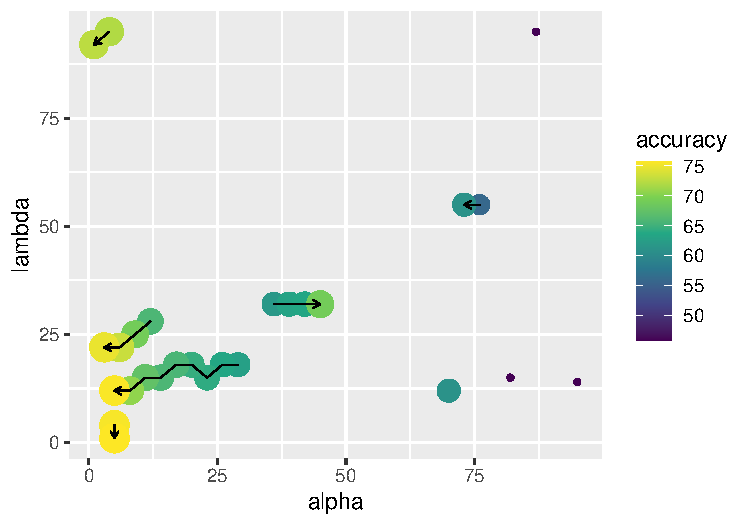
\includegraphics[width=\textwidth]{images/ls}
        \end{center}
    \end{columns}
\end{frame}

%----------------------------------------------------------------------

\begin{frame}{Local Search Considerations}
    \begin{itemize}
        \item Advantages
            \begin{itemize}
                \item Conceptually simple
                \item Adaptive -- later configurations depend on the performance
                    of earlier ones, unlikely to search irrelevant areas
                \item Easily parallelizable
            \end{itemize}
        \item Disadvantages
            \begin{itemize}
                \item Must define local neighborhoods, often needs discretization
                \item Large number of evaluations needed if the starting point is
                    far away from optimum
            \end{itemize}
    \end{itemize}
\end{frame}

%----------------------------------------------------------------------

\begin{frame}{Ablation Analysis}
    \begin{itemize}
        \item Use ``local search'' to determine important hyperparameters
        \item Start from initial configuration (e.g.\ default)
        \item Change configuration, one hyperparameter at a time, until target
            configuration (e.g.\ best found by HPO) is obtained
        \item Choose hyperparameter that has the largest impact on performance
            in each step
        \item Allows to quantify impact of each changed hyperparameter
        \item Does not consider hyperparameter interactions and only evaluates
            local important (specific to the particular pair of configurations)
    \end{itemize}
\end{frame}

\begin{frame}[fragile]{Ablation Analysis Example}
    XGBoost hyperparameter tuning on OpenML dataset 11 (balance-scale)
    \begin{verbatim}
default: 66.56% accuracy
reg_alpha 0.0 -> 2.5595: 73.27999999999999%
learning_rate 0.1 -> 1.3: 75.84%
n_estimators 100 -> 1000: 75.84%
reg_lambda 1.0 -> 1000.0: 76.16%
    \end{verbatim}
    Note interactions between \verb+n_estimators+ and \verb+reg_lambda+ that
    make it appear as if changing \verb+n_estimators+ has no impact
\end{frame}

%----------------------------------------------------------------------

\begin{frame}{Summary} 
\begin{enumerate}
    \item Local Search improves configurations by iteratively looking for
        improvements close to the current best
    \item Ablation Analysis can quantify hyperparameter importance with respect
        to a particular pair of configurations, e.g.\ a default and the best HPO
        has found, but does not consider interactions
\end{enumerate}
\end{frame}

\end{document}
